%%%%%%%%%%%%%%%%%%%%%%%%%%%%%%%%%%%%%%%%%%%%%%%%%%%%%%%
% A template for Wiley article submissions.
% Developed by Overleaf. 
%
% Please note that whilst this template provides a 
% preview of the typeset manuscript for submission, it 
% will not necessarily be the final publication layout.
%
% Usage notes:
% The "blind" option will make anonymous all author, affiliation, correspondence and funding information.
% Use "num-refs" option for numerical citation and references style.
% Use "alpha-refs" option for author-year citation and references style.

\documentclass[alpha-refs]{wiley-article}
% \documentclass[blind,num-refs]{wiley-article}

% Add additional packages here if required
\usepackage{siunitx}
\usepackage{lineno}

% Update article type if known
\papertype{Original Article}
% Include section in journal if known, otherwise delete
\paperfield{Pest Management Science}

\title{Attract and kill: Spinosad baited spheres to control onion maggot (\textit{Delia antiqua})}

% List abbreviations here, if any. Please note that it is preferred that abbreviations be defined at the first instance they appear in the text, rather than creating an abbreviations list.
%\abbrevs{ABC, a black cat; DEF, doesn't ever fret; GHI, goes home immediately.}

% Include full author names and degrees, when required by the journal.
% Use the \authfn to add symbols for additional footnotes and present addresses, if any. Usually start with 1 for notes about author contributions; then continuing with 2 etc if any author has a different present address.
\author[1\authfn{1}]{Denis S. Willett}
\author[1\authfn{1}]{Camila C. Filgueiras}
\author[2]{Starker Wright}
\author[1]{Jan P. Nyrop}
\author[1]{Brian A. Nault}

\contrib[\authfn{1}]{Equally contributing authors.}

% Include full affiliation details for all authors
\affil[1]{Department of Entomology, Cornell AgriTech, Cornell University, Geneva, NY, 14456, USA}
\affil[2]{Bartlett Tree Experts, Dublin, PA, USA}

\corraddress{Denis S. Willett, 15 Castle Creek Drive, Geneva, NY 14456}
\corremail{deniswillett@cornell.edu}


% Include the name of the author that should appear in the running header
\runningauthor{Willett et al.}

\begin{document}

\maketitle

\begin{abstract}

Onion maggot (\textit{Delia antiqua}) is a pest of onions worldwide.  Current means of managing this pest rely heavily on prophylatic insecticide treatments at planting.  These options may not be viable in organic production systems or areas where resistant populations are developing.  Here we explore the efficacy of an attract and kill strategy for control of onion maggot evaluating the ability of attractive, spinosad containing spheres to kill adult onion maggots and reduce field losses.  Spinosad containing spheres were able to consistently kill onion maggot adults over the course of the field season.  Pairing spinosad spheres with Delia Lure increased efficacy of the attract and kill strategy.  Performance of this strategy can reduce damage by onion maggot larvae compared to no insecticide controls, but did not achieved levels of control comparable with insecticide treatment. Implementation of this attract and kill strategy could be a valuable tool in situations where conventional pesticides are not available, where additional control techniques are needed, or for longer term population control of onion maggot.   

% Please include a maximum of seven keywords
\keywords{Onion Maggot, \textit{Delia antiqua}, attraction, sticky-trap, attract-and-kill, lure, onion management}
\end{abstract}

\linenumbers
\section{Introduction}

Allium crops worldwide suffer attack from onion maggot (\textit{Delia antiqua}).  Present in the Americas, Europe and Asia, \textit{Delia antiqua} is well established in most temperate onion growing regions and causes crop losses of up to 100 percent on onions (\textit{Allium cepa} L) if left unmanaged \citep{nault2006performance, nault2006onion}.  Other allium crops including garlic (\textit{Allium sativem} L.), scallions (\textit{Allium fistulosum} L.), and chives (\textit{Allium schoenoprasum} L.) are similarly susceptible\citep{ellis1979factors,ning2017predicting,nault2007ecology, }.  Commercial onion production has relied upon intensive management of this pest, but losses continue to occur in places where crop rotation is not used and resistant populations are present \citep{martinson1988dispersal, nault2006onion}.  

The lifecycle of \textit{Delia antiqua} plays a large role in its severity as an onion pest.  In the northern United States, three generations per year are common \citep{eckenrode1975population, hoepting2004insecticide}.  While adults can be captured in fields using sticky cards, the larvae cause devastating damage through feeding on plant roots and onion bulbs \citep{nault2006onion, nault2006performance}. Feeding by onion maggot larvae early in the season can kill seedlings and damaged plants can become more susceptible to infection by pathogen and attack by subsequent generations \citep{eckenrode1986impact,nault2006performance}.  Feeding by onion maggot larvae, even if it does not completely kill the onion can cause sufficient damage to prevent sale of the produce.   

Prophylatic insecticide applications at planting are the current tool of choice to manage this pest \citep{nault2006performance}.  The seed treatment package containing thiamethoxam, spinosad and several fungicides (FarMore FI500) is commonly used as is a cyromazine seed treatment with Chlorpyrifos drench \citep{nault2006performance}.  Crop rotation, removal of damaged onions, and delayed planting can all be used to reduce onion maggot damage, but may not be the strategy of choice for large scale commercial growers \citep{martinson1988dispersal, finch1985influence, nault2011delaying}.   

Management of this pest has relied on prophylactic insecticide applications at planting \citep{nault2006performance}.  A variety of organophosphate and carbamate insecticides have been used and discontinued \citep{nault2006performance}.  Chlorpyrifos is commonly used as a drench treatment in combination with either cyromazine seed treatment (Trigard)  \citep{nault2006performance} or the seed treatment package containing thiamethoxam, spinosad and several fungicides (FarMore FI500).  Cultural practices such as crop rotation, removal of damaged onions, and delayed planting are also effective management tactics \citep{martinson1988dispersal, finch1985influence, nault2011delaying}.  

Recent efforts in monitoring onion maggot populations, however, have opened the possibility of a new control strategy for \textit{Delia antiqua}.  Onion maggot adults respond to and are attracted by visual and chemical cues \citep{harris1983color,harris1988host, thomingdeveloping, otto2000development}.  Visually, onion maggot adults tend to prefer large white spheres, while chemically they respond strongly to chemical constituents of decomposing onion.  In particular, two components of decomposing onion, 2-phenyl-ethanol and n-valeric acid, are attractive and have been formulated into attractive lures \citep{ishikawa1984mixture,ishikawa1987controlled, kuhar2006field}.  Combining the white spheres with the chemically attractive lures approximately doubled onion maggot trap catch \citep{willett2019}.  Adding an insecticide to these attractive spheres could be an effective attract and kill solution for controlling onion maggot.  

Attract and kill strategies rely on pairing an attractive component, usually involving a semiochemical and/or visual component, with a killing component whether through mechanical or chemical means \citep{gregg2018advances}.  Attract and kill strategies can be more specific and environmentally friendly and have contributed to integrated pest management of flies and moths \citep{gregg2018advances}.  Of particular interest and inspiration for this work, red insecticide treated spheres have been developed as an attract and kill solution for control apple maggot in northeastern orchards \citep{bostanian2001attract,duan1995control}.  

Of particular consideration in developing an attract and kill solution for use in an integrated pest management program is choice of the killing component of the package.  For working with onion maggot control, we elected to use Spinosad as an insecticidal killing component.  Spinosad is a naturally derived neurotoxic insecticide originally isolated from the soil dwelling actinomycete \textit{Saccharopolyspora spinosa} \citep{racke2007reduced}.  It has been approved for use on over 150 fruit and vegetable crops in the United States and is certified for use in organic production by the USDA National Organic Standards Board and Organic Materials Review Institute (OMRI) \citep{racke2007reduced,williams2003naturally}.  In addition, spinosad has substantially lower non-target effects relative to conventional pesticides and low residual toxicity \citep{williams2003naturally}.  Because of its complementary nature to current conventional management of onion maggot and potential use in organic production systems, spinosad was included in development of an attract and kill solution for onion maggot.  

To develop an effective attract and kill solution to control onion maggot, we combined attractive white spheres developed in previous work \citep{willett2019} with a spinosad insecticide solution and evaluated the ability of these spinosad attractive spheres to kill adult onion maggot flies and reduce damage to onions over the course of three field seasons in upstate New York.  

\section{Materials and Methods}

Field trials evaluating the efficacy of attract and kill strategies to manage onion maggot populations were conducted from 2006 to 2008 in commercial dry bulb onion fields on muck soils in upstate New York.  Muck soils are high organic matter soils formed from old lake beds.  Trials were conducted from May to September.  

\subsection{Population Monitoring}

Population monitoring of onion maggot adults was accomplished by deploying white sticky cards in triplicate with six replications in control areas of experimental plots deployed using a randomized controlled block design.  Cards were collected weekly from May to September and the number of male and female adult flies counted.  

\subsection{Onion Maggot Mortality}

Because white spheres has previously been shown to be attractive to onion maggot adults, 1\%, 0.5\%, and 0\% (control) spinosad were added to paraffin and coated on 8.75cm diameter white plastic spheres to evaluate the ability of the spheres to cause onion maggot mortality.  Additionally, the temporal efficacy of the spinosad solution was evaluated.  

To do so, the ability of spinosad spheres to kill onion maggot flies was evaluated over the course of multiple field seasons by deploying a cohort of spheres containing spinosad at the beginning of the season (mid May) and recovering a subset of them on a monthly basis to evaluate climate and dose effects.  Spheres had three levels of spinosad: No Spinosad (Control), 0.5\% Spinosad, and 1\% Spinosad.  Following initial deployment in mid May spheres were recovered in mid June, mid July, mid August, and mid September resulting in cohorts exposed to field conditions for 1 month, 2 months, 3 months, 4 months, respectively.  Deployment in the field followed a randomized controlled block design.

Following recovery from the field, spheres were photographed to document degradation, then immediately suspended in ~25cm x 25cm x 50cm screen and plexiglass cages containing water in a petri dish. Ten male and ten female onion maggot flies were then introduced to each cage and mortality monitored every 24 hours for 72 hours.  This trial was conducted for both spinosad  containing and control spheres.  Six replications of each treatment, exposure combination was conducted.  

\subsection{Field Damage}

To evaluate the efficacy of attract and kill techniques in controlling onion maggot damage, field damage from onion maggot larvae was monitored throughout the season.  Onion seed of \textit{Allium cepa} L. 'Arsenal', an early yellow globe variety, was planted in late April with plants subjected to six treatments in a randomized controlled block design.  Insecticide treated plants were treated at planting with a seed treatment package package containing thiamethoxam, spinosad and several fungicides (FarMore FI500).  This was placed in the experiment to be a positive control.  No insecticide treated plants did not receive the seed treatment package and did not receive any attract and kill strategies.  Spinosad spheres containing 0.5\% spinosad were deployed with and without attractive Delia Lures (AgBio, Westminster, CO) as and attract and kill solution.  White sticky cards with and without attractive Delia Lures were also deployed.   Four replications of each treatment combination were evaluated.  

Each individual experimental plot was 8 rows by 30 feet long separated from its nearest neighboring experimental plot by a minimum of 100 feet in any direction.  Three weeks following planting, seedlings in the middle two rows were counted to obtain an initial stand count.  Following initial stand count, plant loss due to damage by onion maggot larvae was evaluated on a weekly basis in the middle two rows until the end of season when a final stand count was taken (including all mortality factors).  Plant loss due to onion maggot was assessed visually then confirmed by removing the plant and ascertaining presence of onion maggot larvae.  

\subsection{Enhanced Formulation}

To enhance attractiveness, longevity, and performance of spinosad baited spheres, a new formulation of spinosad containing sphere was developed with 0.5\% spinosad, 5.0\% ammonium carbonate and 5.0\% casein hydrolysate.  The efficacy of this new formulation was compared to spheres containing just 0.5\% spinosad and no spinosad controls in field cage trials.  Treatments were deployed in a randomized controlled block design with four replications and each individual plot consisting of four rows on onion by 30ft long.  Plots were seeded in early May and each plot was caged using PVC pipe and screen mesh.  One hundred fifty adult flies with a 50:50 male to female ratio were released into each cage on the second of June and nine days later on June 11th.   As described above, Initial and final stand counts were taken and plant damage due to onion maggot larvae evaluated on a weekly basis.  


\subsection{Analysis}

To evaluate population dynamics of onion maggot over time, a smoothing function consisting of a generalized additive model with cubic splines was fitted to the raw population numbers for visual display.  

To evaluate adult onion maggot mortality as a result of contact with spheres containing spinosad, linear models and analysis of variance were used.  Models were determined after consideration of all factor combinations and interactions and selected based on consideration of residual diagnostics (conformance to assumptions of normality and homoscedasticity), goodness of fit tests, $R^2$ values, information criteria, and leverage considerations. Main effects were teased out from interactions using Tukey and Dunnett post-hoc tests.  

Field damage and stand loss were evaluated using mixed effects linear and negative binomial models.  Best fit models were selected after consideration of data distributions, residual diagnostics, likelihood ration considerations, information criteria, and psuedo-$R^2$ values, root mean squared error and coefficient of variation of root mean squared error.  


\subsection{Data Management}

All data for the trials were entered into flat tabular (.csv) files.  All analysis on the raw data was conducted in R version 3.5.2 using RStudio as an IDE (with Vim keybindings) \citep{rcore2018,rstudio}.  The $tidyverse$, $car$, $lme4$, and $emmeans$ packages were used to facilitate analysis \citep{tidy, car, lme, emmeans}.  All code, including manuscript documentation, is available on GitHub (https://github.com/acetworld/onion-maggot-control).


\section{Results}

\paragraph{Population Monitoring}

During the field seasons monitored in these trials in upstate New York, \textit{Delia antiqua} had three generations (Figure \ref{fig:figure1}).  The first population of adults peaked in June, the second in late July, and the third in August.  More males than females were collected on sticky cards, but both males and females followed roughly the same population cycles. 

\paragraph{Onion Maggot Mortality}

White spheres baited with spinosad caused appreciable mortality of onion maggot adults (Figure \ref{fig:figure2}A).  Both spinosad rate (F =114.3, df=2, p \textless 0.001)  and exposure time (F = 4.7, df = 1, p = 0.03) in the field significantly explained approximately 62\% of the observed variation in adult onion maggot mortality ($R^2_{adj}$ = 0.62, p \textless 0.001).  Both rates of spinosad treated spheres caused approximately 47$\pm$4\% more onion maggot mortaliy than untreated controls (Figure \ref{fig:figure2}B).  Increasing rates of spinosad from 0.5\% to 1\% did not signifcantly increase onion maggot mortality (Figure \ref{fig:figure2}B).  

Increasing time spent in the field did tend to decrease efficacy of spinosad containing spheres (Figure \ref{fig:figure2}C).  For every month of exposure, mortality of onion maggot tended to decline 3$\pm$1\%.  After four months of exposure, and despite obvious degradation of the parafin containing the spinosad (Figure \ref{fig:figure2}D), onion maggot mortality as a result of contacting spinosad baited spheres still remained above 45\% (Figure \ref{fig:figure2}C).  

Onion maggot mortality as a result of contacting spinosad containing spheres was not constant over the 72 hours of monitoring in cages (Figure \ref{fig:figure3}).  For both spinosad rates, onion maggot mortality tended to peak at around 48 hours for spheres with one month exposure to field conditions (the June cohort).  After longer exposure to field conditions, onion maggot mortality tended to decline over the course of 72 hours.  

\paragraph{Field Damage}

Deployment of the attract and kill solution of spinosad baited spheres did not substantially affect end of season onion loss as a result of all mortality factors (Figure \ref{fig:figure4}A), but did influence cumulative damage as a result of onion maggot larval feeding (Figure \ref{fig:figure4}B).  Treatment solution (Insecticide, No Insectide, Spinosad Sphere, Sticky Card) significantly (F = 5.8, df = 3, p = 0.005) explained approximately 38\% of the observed variation in end of season onion stand loss as a result of all mortality factors ($R^2_{adj}$ = 0.38, p = 0.005, Figure \ref{fig:figure4}A).  The presence of Delia Lure did not significantly (p \textgreater 0.05) affect end of season onion stand loss.  Insecticide treatment worked best at preventing end of season stand loss (Figure \ref{fig:figure4}A).  The no insecticide treatment was highly variable and not significantly (p \textgreater 0.05)  different from insecticide controls.  Spinosad and sticky card treatments were not significantly different from no insecticide treatments, but were significantly worse than insecticide controls. 

Cumulative damage as a result of onion maggot larval feeding was significantly explained by treatment solution ($\chi^2$ = 42.2, df = 3, p \textless 0.001), the presence of Delia Lure ($\chi^2$ = 10.0, df = 1, p = 0.001), and their interaction ($\chi^2$ = 21.4, df = 1 p \textless 0.001).  Cumulative damage due to feeding by onion maggot larvae over the course of the field seasons ranged from 0 in some control plots to 82 dead onion maggot plants in a few plots. This amounts to approximately 20-30\% losses of onion directly attributable feeding by onion maggot larvae.  All treatments were significantly worse than insecticide controls which had very low levels of onion maggot damage (Figure \ref{fig:figure4}B).  Pairing Delia Lure with spinosad containing spheres significantly reduced damage by onion maggot larvae by 72$\pm$10\% (p \textless 0.001) compared to spinosad spheres alone.  Pairing Delia Lure with sticky cards had the opposite effect (Figure \ref{fig:figure4}B).  

\paragraph{Enhanced Formulation}

Treatment significantly explained observed onion maggot damage in field cage trials with the enhanced formulation ($\chi^2$ = 23.9, df = 2, p \textless 0.001).  The enhanced formulation (Spinosad +) containing 0.5\% spinosad, 5.0\% ammonium carbonate and 5.0\% casein hydrolysate did not perform significantly different than Spinosad only treatments with 0.5\% spinosad containing spheres.  Both treatments containing spinosad performed significantly better than No insecticide controls (p \textless 0.05).  


\begin{figure}[bt]
\centering
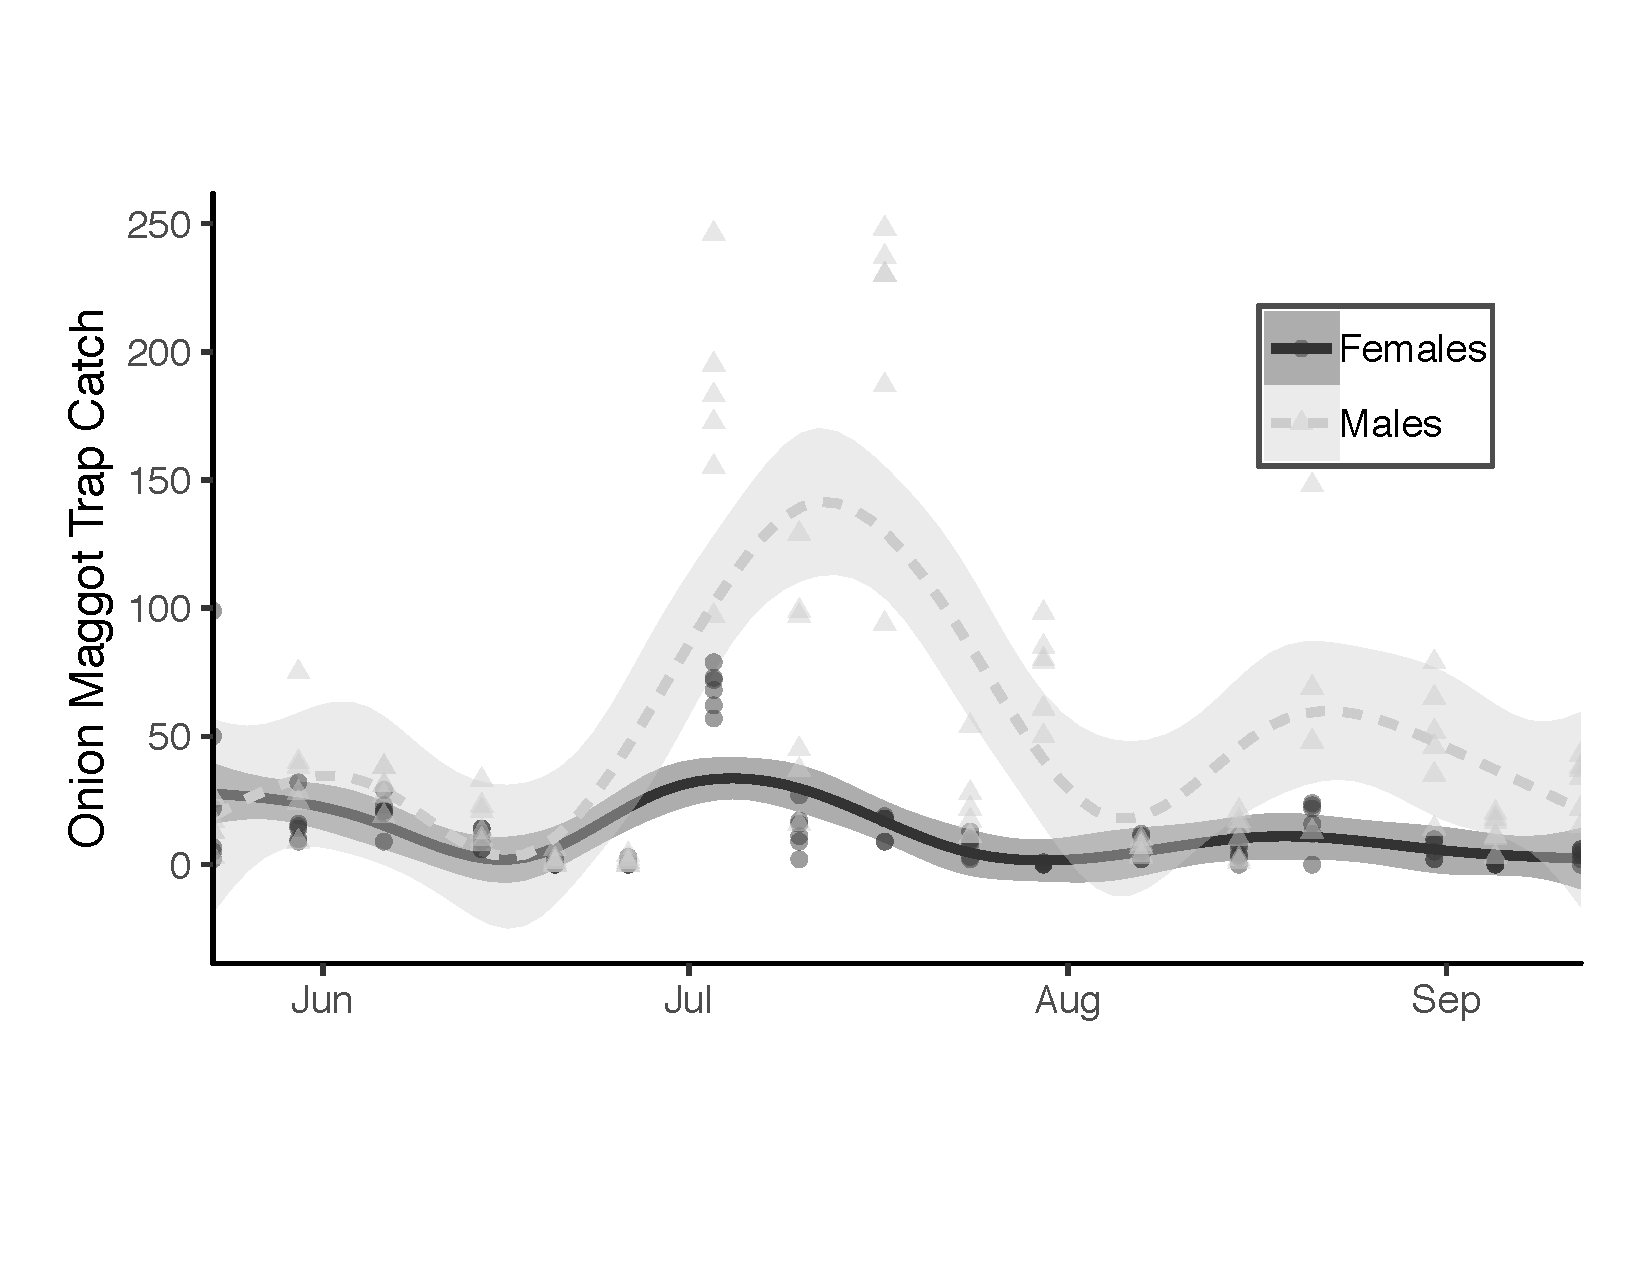
\includegraphics[width = 8cm]{figures/final-figures/figure-1.pdf}
\caption{Population dynamics of adult onion maggot (\textit{D. antiqua}) flies in upstate New York muck regions.  Points indicate observations of numbers of adult flies captured on sticky cards.  Lines and shaded regions indicate smoothed fits and 95\% confidence intervals respectively.  }
\label{fig:figure1}
\end{figure}

\begin{figure}[bt]
\centering
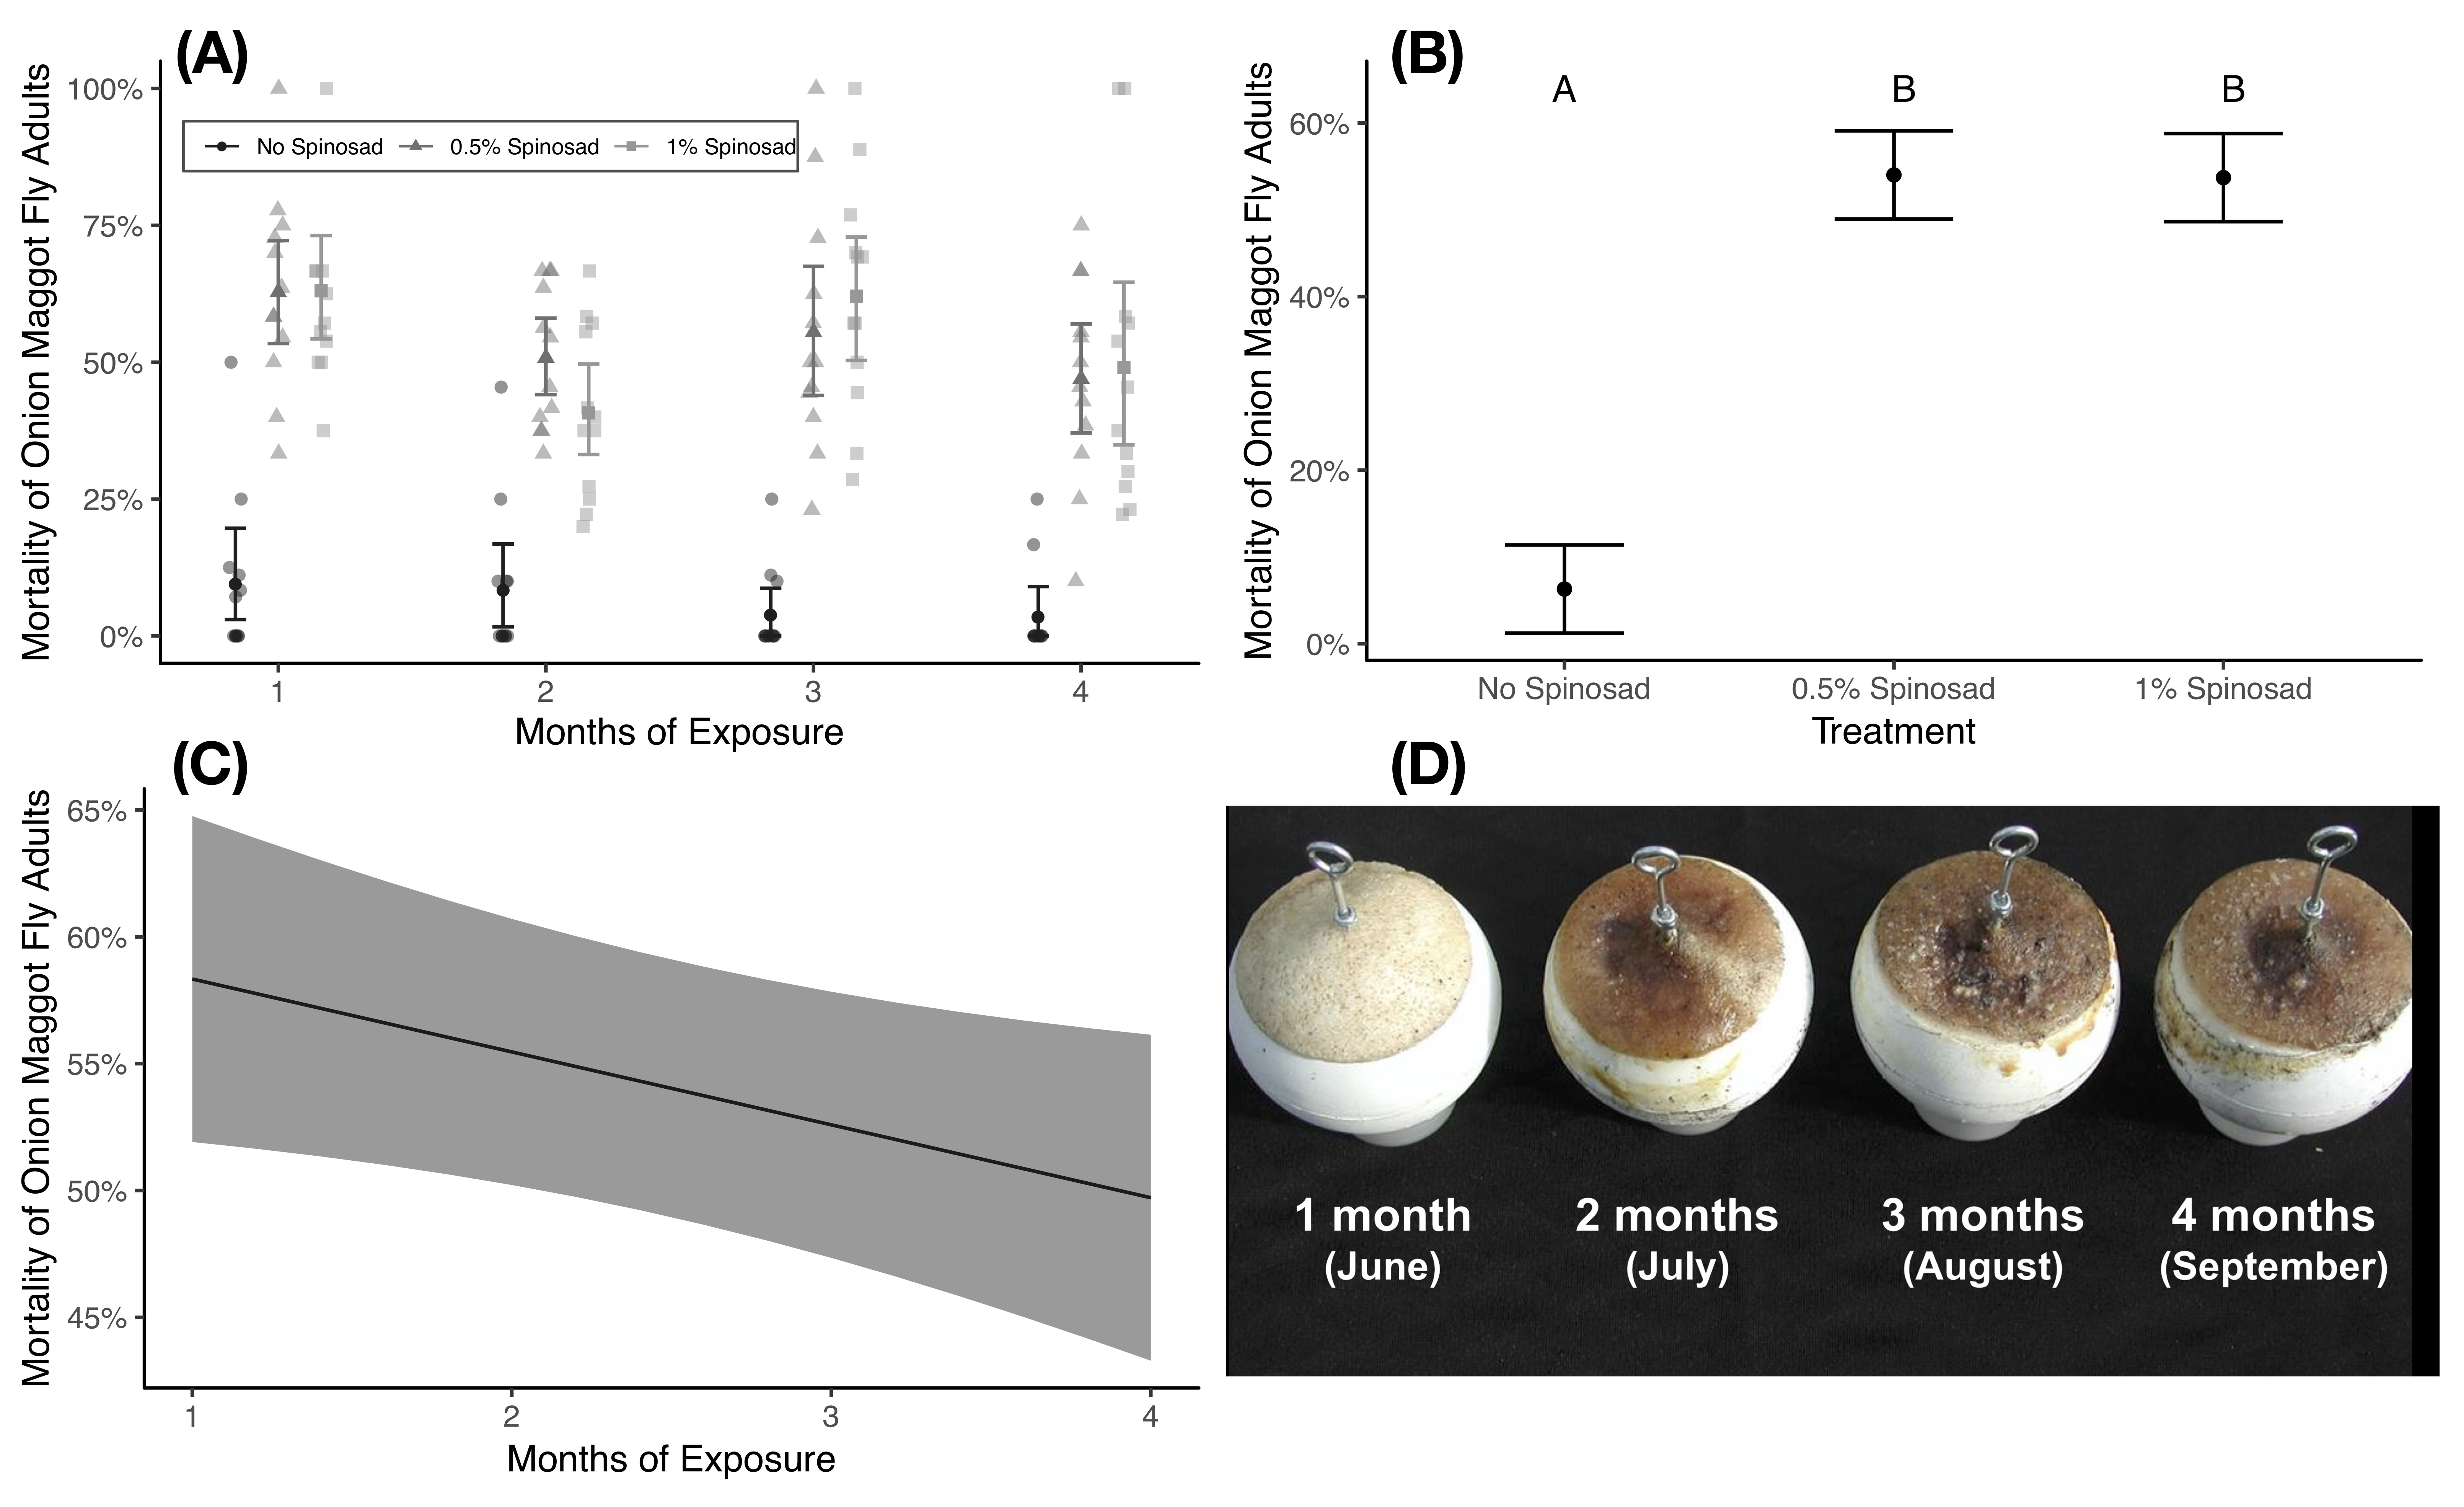
\includegraphics[width = 8cm]{figures/final-figures/figure-2.pdf}
\caption{Adult onion maggot (\textit{D. antiqua} mortality in the presence of spinosad treated spheres.  (A) Raw data of effects of exposure time and spinosad rate on mortality of adult onion maggot flies.  Light points indicate individual observations.  Solid points and error bars denote mean and 95\% confidence intervals respectively.  (B) Main effects of spinosad rate on adult onion maggot mortality.  Points and error bars denote mean effect and 95\% confidence intervals respectively.  Different letters denote significant differences (p \textless 0.05).  (C) Main effect of exposure time on adult onion maggot mortality.  Line and shaded area denote effect and 95\% confidence region respectively.  (D) Photographs of spinosad treated spheres at increasing exposure time in field conditions.  Spheres were placed in the field on the 15th of May.  }
\label{fig:figure2}
\end{figure}


\begin{figure}[bt]
\centering
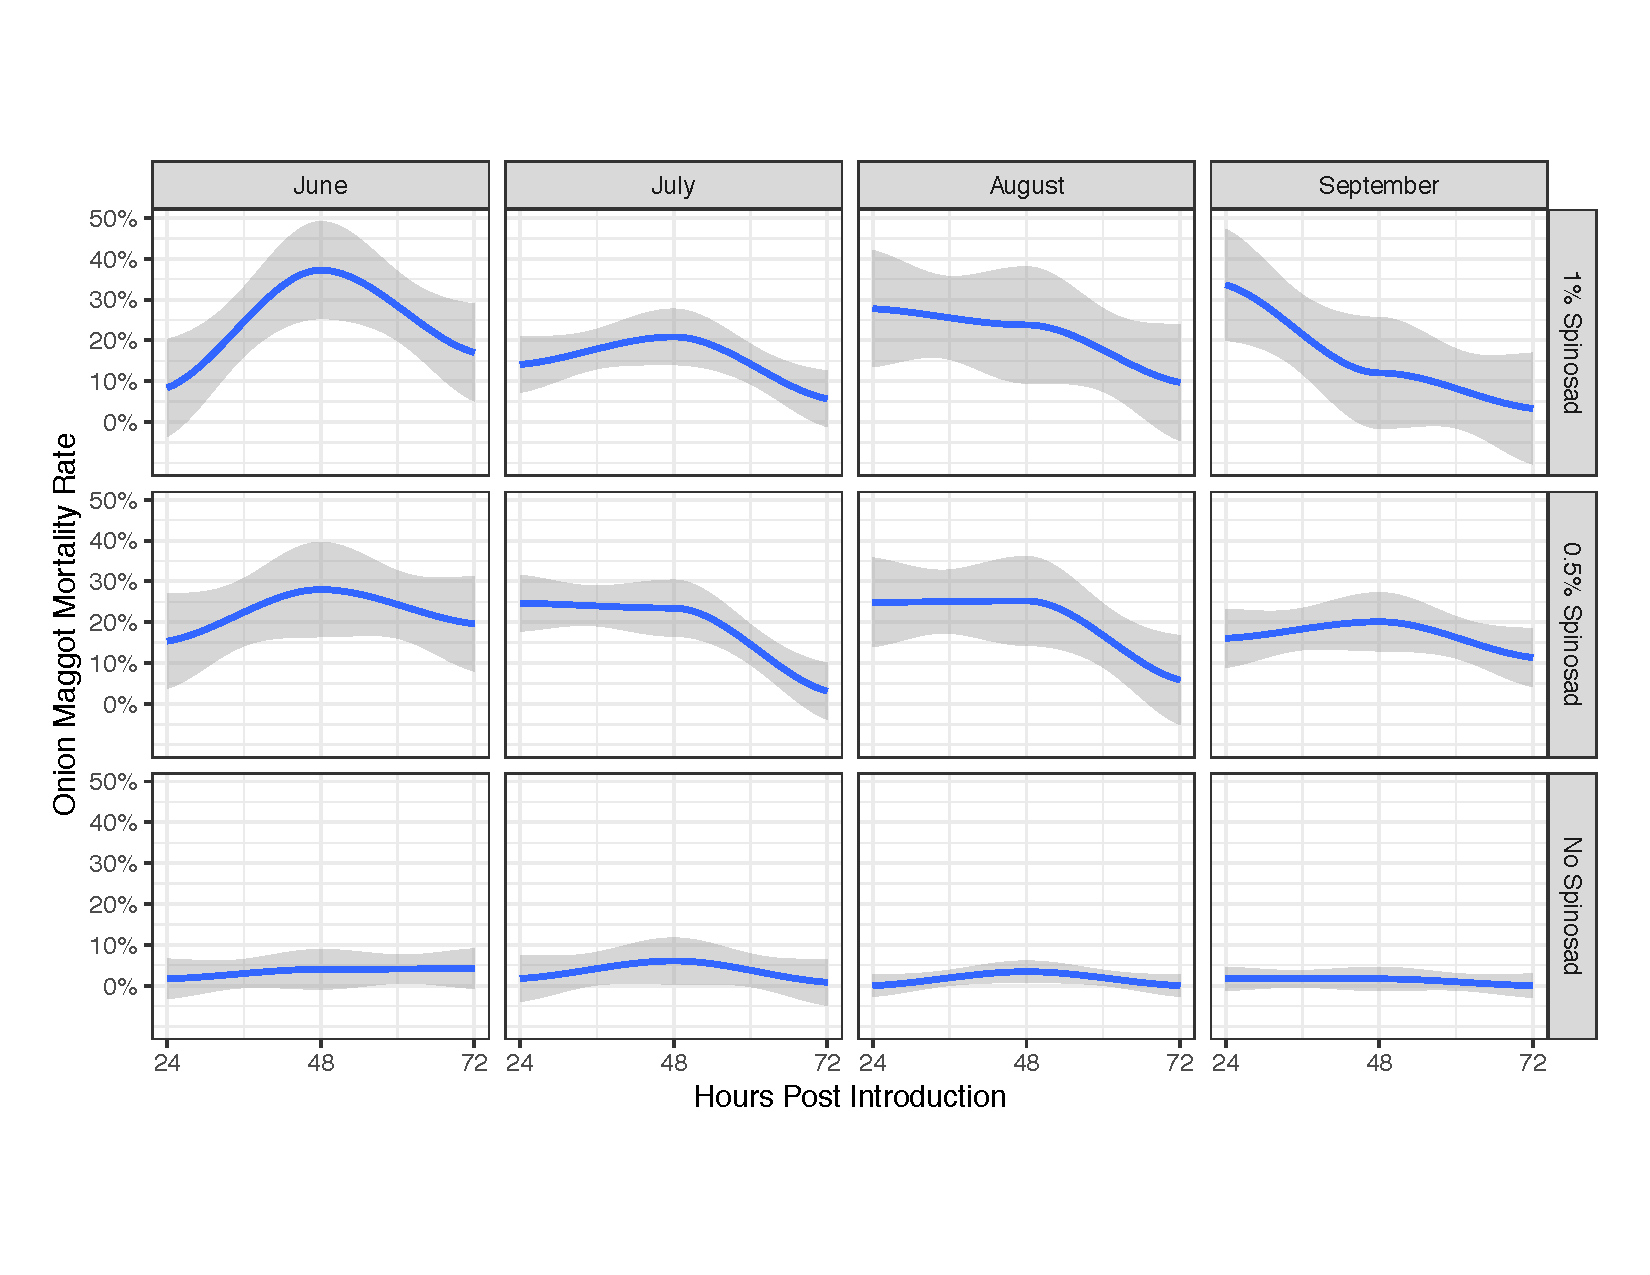
\includegraphics[width = 8cm]{figures/final-figures/figure-3.pdf}
\caption{Adult onion maggot fly mortality following introduction to cages containing spinosad treated spheres.  Spheres were treated with differing rates of spinosad (rows) and exposed to field conditions for increasing amounts of time (column).  Lines and shaded regions indicate fitted smoothed (LOESS) mortality rates and 95\% confidence regions respectivel.  }
\label{fig:figure3}
\end{figure}


\begin{figure}[bt]
\centering
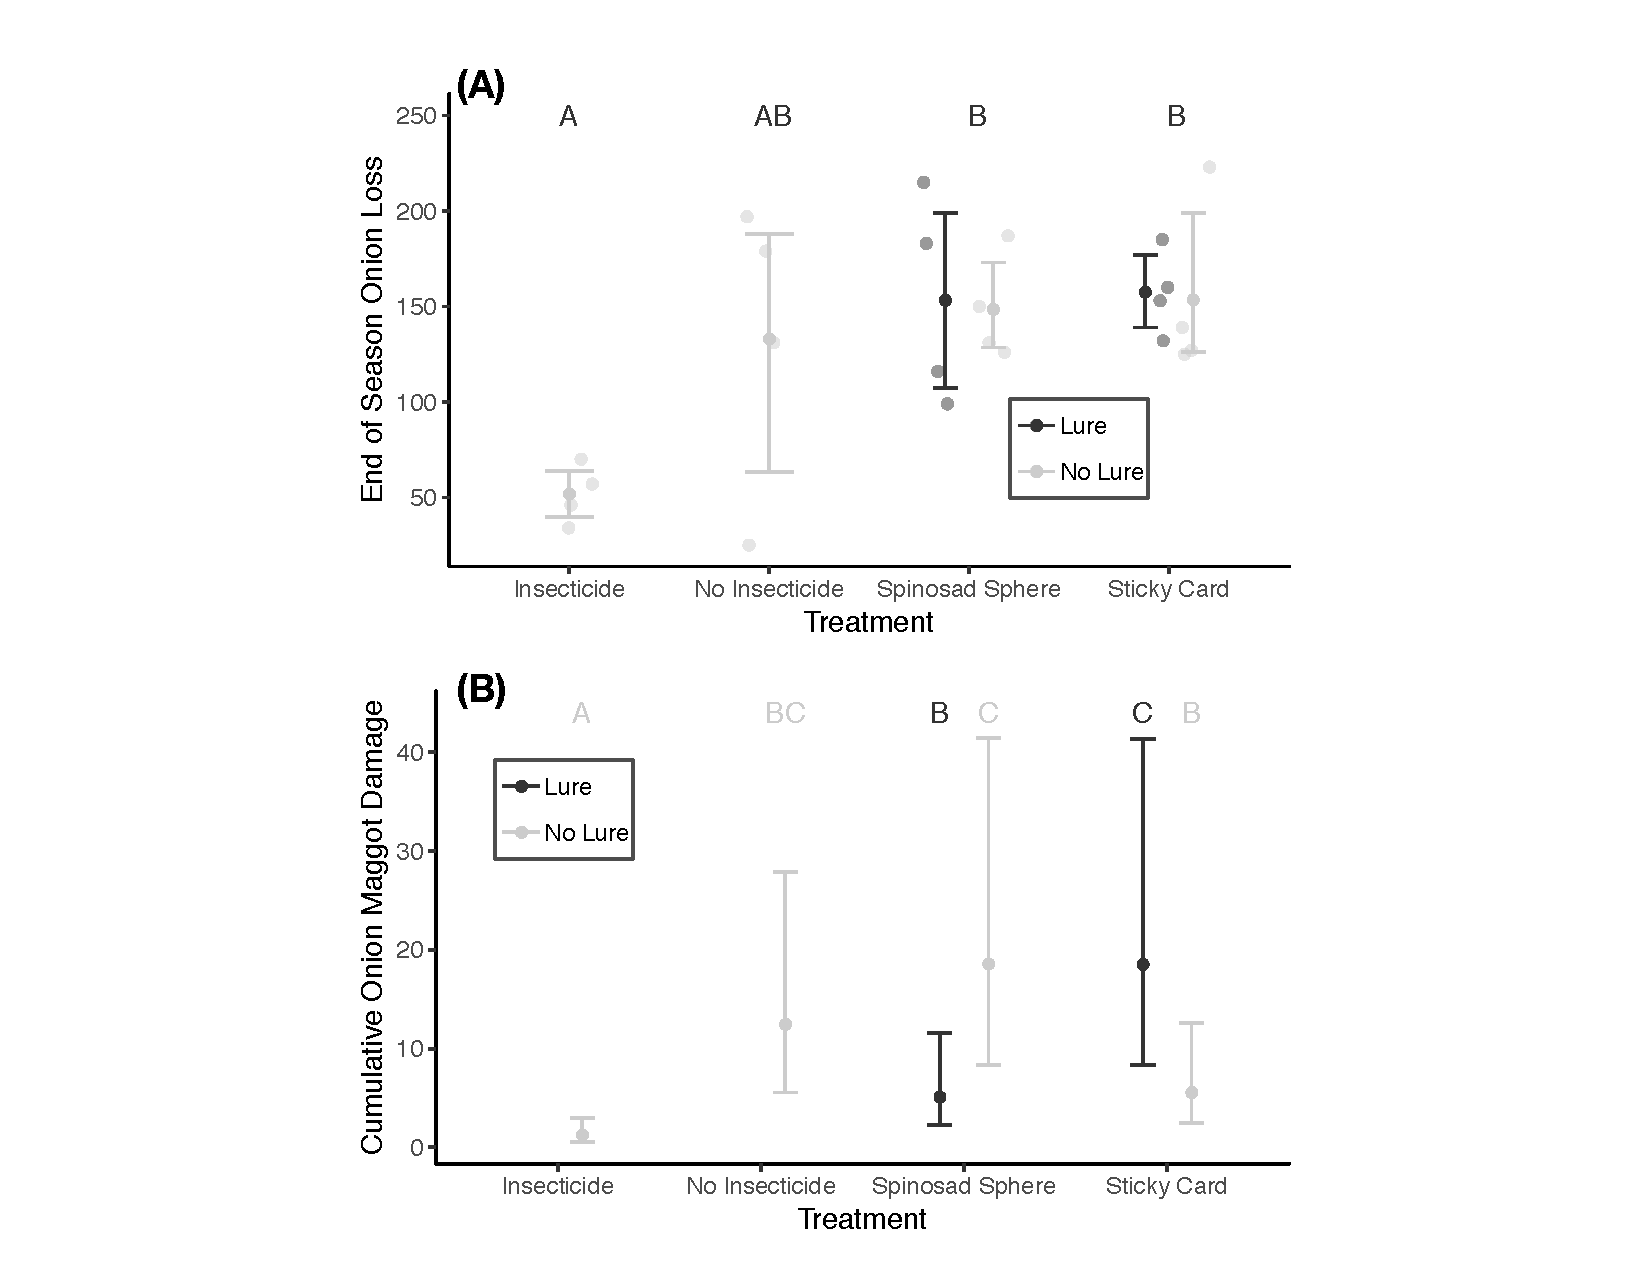
\includegraphics[width = 8cm]{figures/final-figures/figure-4.pdf}
\caption{Field damage of onions.  (A) End of season stand loss of onions (number of dead onion plants) as a result of all mortality factors.  (B) Cumulative damage (number of dead onion plants) as a result of onion maggot larval feeding.  Light points indicate observed values.  Solid points and errorbars denote mean effects and 95\% confidence intevals respectively.  Different letters denote significant differences (p \textless 0.05).   }
\label{fig:figure4}
\end{figure}


\begin{figure}[bt]
\centering
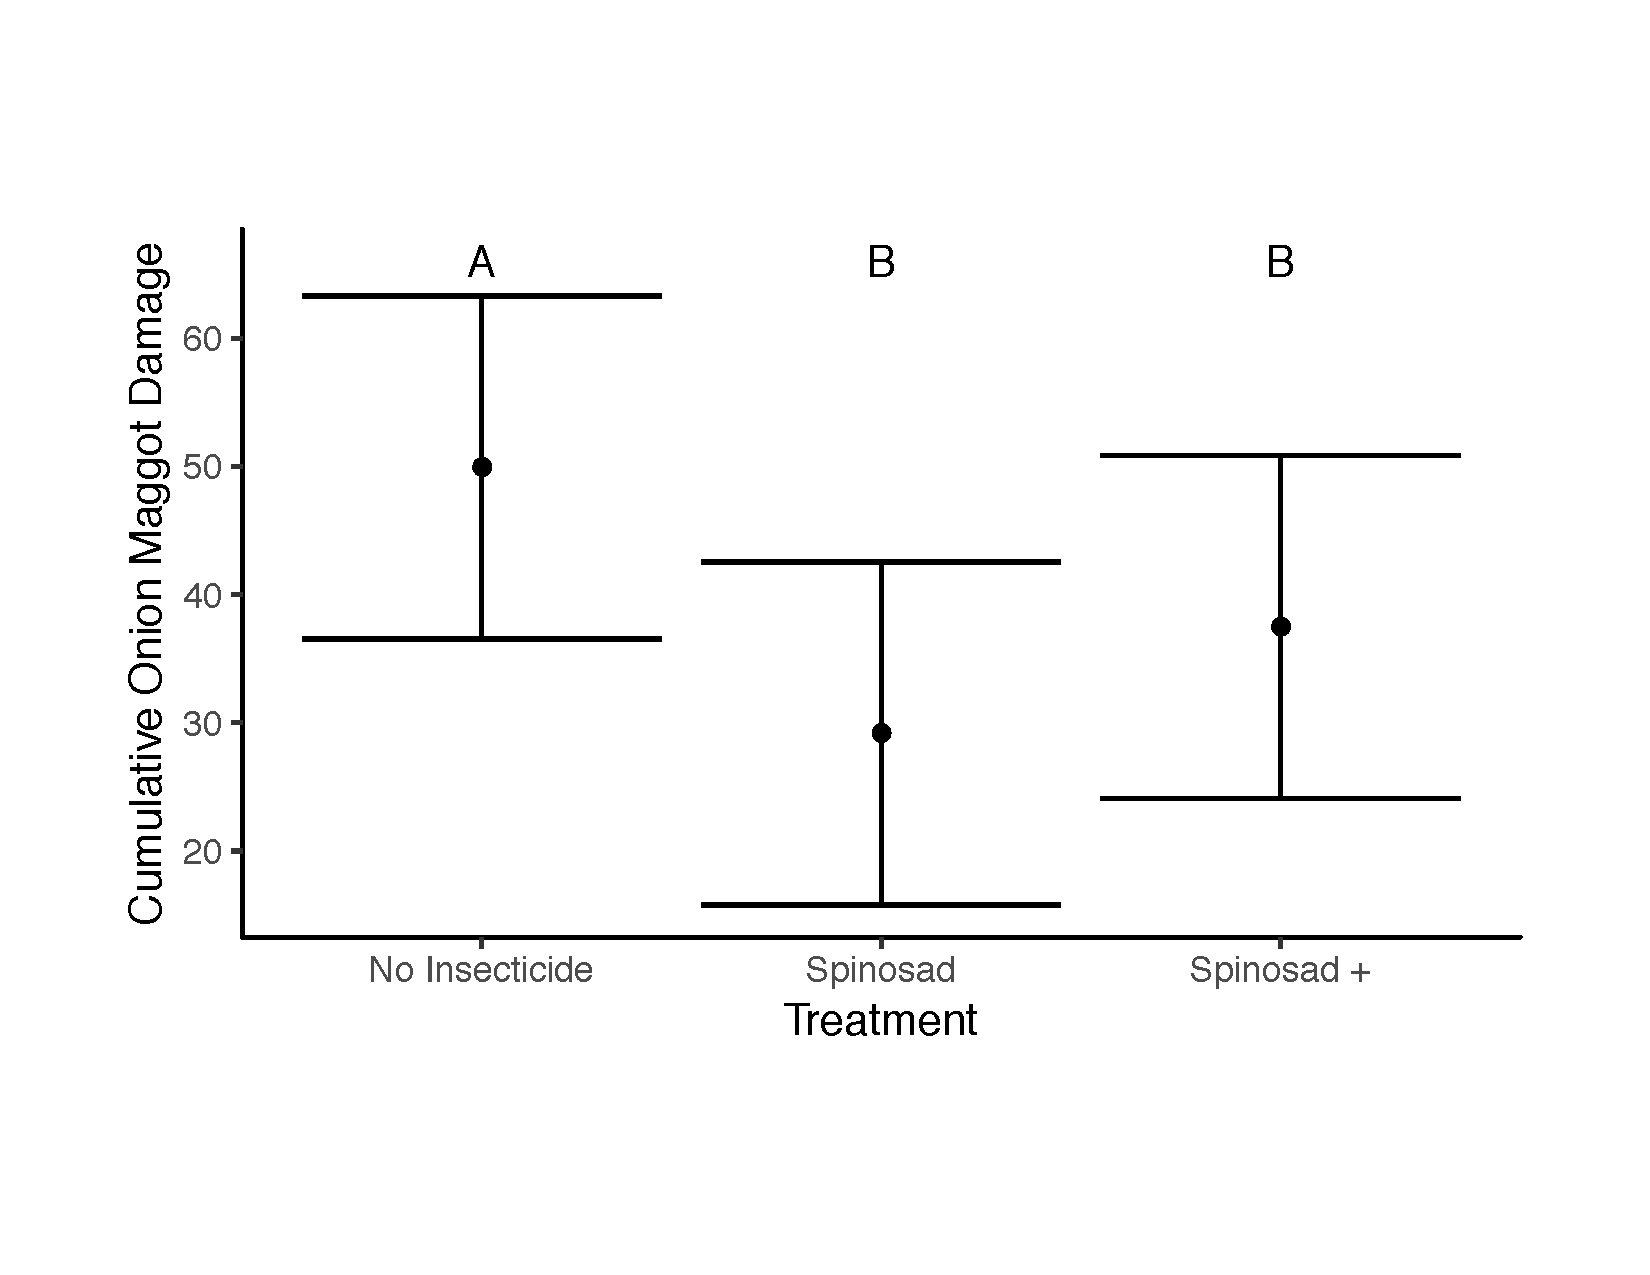
\includegraphics[width = 8cm]{figures/final-figures/figure-5.pdf}
\caption{Field damage of onion in enclosed cages with differing spinosad sphere formulations.  Cumulative damage is number of dead plants as a result of onion maggot damage.  Points and error bars denote mean and 95\% confidence intervals respectively.  Different letters denote significant differences (p \textless 0.05).  }
\label{fig:figure5}
\end{figure}





\section{Discussion}

Using spinosad baited spheres as an attract and kill solution for control of onion maggot populations may be an effective tool under an integrated pest management approach.  Over the course of the three field seasons, with three generations per year (Figure \ref{fig:figure1}), the attract and kill solution was able to consistently inflict mortality on adult onion maggot flies, even after prolonged exposure to field conditions (Figure \ref{fig:figure2}).  While exposure did tend to reduce efficacy (Figure \ref{fig:figure2}C) and change the dynamics of mortality (Figure \ref{fig:figure3}), any effects were marginal and may be due to melting of the paraffin solution containing the spinosad (Figure \ref{fig:figure2}D).  

Importantly for practical use of this technique, higher doses of spinosad did not have noticeable effects on onion maggot mortality.  The low rate of spinosad containing spheres resulted in adult onion maggot mortality that was not significantly different than mortality resulting from contact with spheres containing higher levels of spinosad (Figure \ref{fig:figure2}B).  This suggests that inclusion of spinosad as the insecticide component of this attract and kill technique was not only an effective choice for implementation of an attract and kill strategy, but also is a viable option even at low doses.  

Using field onion maggot population averages and mortality achieved by spheres over time, numbers of adult onion maggots killed as a result of the attract and kill strategy can be estimated. During peak flights, approximately 272 onion maggot adults (both males and females) were caught on average per week.  Over the course of the field season, approximately 64 adults were caught by sticky cards on average per week.  Assuming spinosad baited spheres kill approximately 54\% of the adults they contact, over the course of a 16 week season, this attract and kill solution could have killed approximately 553 onion maggot adults (16 weeks x 64 adults on average per week * 0.54 mortality) per spinosad containing sphere.  

Although spinosad containing spheres were able to kill large numbers of onion maggot adults, the attract and kill solution did not appreciably affect end of season onion loss when all mortality factors were considered.  These other mortality factors include climatic effects, pathogen infection, and attack by other insect pests such as onion thrips.  The attract and kill solution did appreciably affect onion mortality due to feeding by \textit{Delia antiqua} larvae, however.  

The juxtaposition of these two results baselined against insecticide positive control and no insecticide negative controls suggests that insecticide treatments may be reducing other mortality factors in addition to controlling some damage by onion maggot larvae.  Spinosad spheres in conjunction with the attractive Delia Lure resulted in levels of damage almost as good as insecticide controls, but with variation that led to overlap with no insecticide negative controls.  In caged field trials, spinosad spheres reduced damage resulting from onion maggot feeding to below that of no insecticide controls.  Interestingly, pairing Delia Lure with sticky cards produced higher levels of damage.  This is likely because the kill part of the attract and kill sticky card solution was ineffective; delia lures likely attracted adult fly populations to plots but sticky cards did not cause sufficient mortality.  Augmenting spinosad spheres with ammonium carbonate and casein hydrolysate did not appreciably change control with this attract and kill method.  

While not as effective as insecticide controls, using this attract and kill approach with spinosad spheres may be a choice where other options are not viable or as a complementary tool in an integrated pest management program.  Spinosad spheres do cause adult onion maggot mortality over extended field seasons.  In situations where immediate reduction in damage from onion maggot is desired, this attract and kill approach may be desired in situations where conventional insecticide management is not available either with resistant populations or in organic production systems.  Additionally, this attract and kill approach could be used as a control option where conventional pesticides are no longer effective or available. This strategy could also hold promise as an additional mortality factor in longer term management to control onion maggot populations.  

\section*{Acknowledgements}
We appreciate technical assistance by M. Hessney and Delia Lure contributions from J. Meneley. The New York State Integrated Pest Management Program, USDA/CSREES Pest Management Alternatives Program, and New York State Department of Agriculture and Markets Onion Research and Development Program supported this research. 

\section*{Conflict of Interest}
The authors declare no conflict of interest.  

\section*{Author Contribution}
BAN, JPN, and SW designed the experiments.  DSW, CCF, and BAN analyzed the data and wrote the manuscript.  


\section*{Data Availability Statement}
All code and data, including manuscript documentation, is available on GitHub(https://github.com/acetworld/onion-maggot-control).

%\printendnotes


\section{References}

\bibliographystyle{vancouver-authoryear}
\bibliography{om-attraction}

\graphicalabstract{example-image-1x1}{Please check the journal's author guildines for whether a graphical abstract, key points, new findings, or other items are required for display in the Table of Contents.}

\end{document}
